%This is a template file for use of iopjournal.cls

\documentclass{iopjournal}

% Options
%  [anonymous]  Provides output without author names, affiliations or acknowledgments to facilitate double-anonymous peer-review
%
% The following packages are required by iopjournal.cls and do not need to be declared again:
%  graphicx
%  fancyhdr
%  xcolor
%  hyperref
%
\begin{document}

\articletype{Journal Article} %	 e.g. Paper, Letter, Topical Review...

\title{Automated Age Prediction of White-tailed Deer via Deep Learning and Computer Vision}

\author{Aaron J. Pung, Ph.D.$^{1,*}$}

\email{aaron.pung@gmail.com}

\keywords{machine learning, computer vision, neural network, deer, age, classification, prediction, dental analysis, tooth wear, wildlife, management, automation, assessment}

\begin{abstract}
Accurate age estimation of white-tailed deer (\textit{Odocoileus virginianus}) is critical for understanding herd dynamics and informing management decisions. This study describes two computer vision models to predict deer age from trail camera imagery and jawbone photographs. Using transfer learning with convolutional neural networks, the trail camera model achieved $78.4\%$ accuracy and the jawbone model achieved $90.7\% \pm 2.6\%$ accuracy on held-out test data. Both models significantly outperformed traditional classifiers ($57.3\%$), human expert assessment ($58.6\%$), morphometric methods ($63\%$), and the $70\%$ accuracy threshold required for professional wildlife management. Attention map analysis confirmed that models identified biologically relevant age-related morphological features rather than spurious correlations. These automated methods provide rapid, objective age determination with immediate practical applications for wildlife agencies, research institutions, and harvest monitoring programs.
\end{abstract}

\section{Introduction}
Characterizing white-tailed deer populations is crucial to measuring their impact on ecosystems, human health, and property. Herd health, for instance, informs management decisions like hunting regulations, disease response, and protection against environmental damage from overgrazing. As a result, age-related data is becoming increasingly important since deer age affects body growth, doe fertility, antler quality, and sex ratios of offspring.

State-of-the-art trail cameras enable hunters and professionals to monitor the movement and health of local deer populations, but estimating the age of white-tailed bucks from camera imagery remains challenging. One technique known as "Aging On The Hoof" (AOTH) attempts to determine age by analyzing the location and date of each image as well as the relative body proportions of the buck in the image \cite{1996Kroll, 1978Knowlton, 1999Demarais, 2003Richards, 2008Hellickson}. When the buck's body measurements are not known, human AOTH estimate averages just 36\% -- less than half the accuracy required for management-related selective harvest decisions ($\geq70\%$) or research purposes ($\geq80\%$) \cite{2014Gee}. 

%However, when the buck's body measurements are known, morphometric models can be used to achieve a prediction accuracy of 63\% during post-breeding periods \cite{2010flinn}. More recent efforts have achieved significantly greater prediction accuracy (76.7\%) by applying computer vision (CV) and deep learning (DL) to trail camera imagery \cite{2025pung}, providing the first automated approach that meets the accuracy thresholds necessary for practical wildlife management applications.

%As machine learning (ML) and computer vision (CV) become more engrained in societyare With the dawn of AI and ML, ... with existing computer vision methods limited to trail camera imagery and manual dental analysis requiring specialized expertise.

%Sample text inserted for demonstration. Organize the main text of your article using section headings, and include any equations, figures, tables, lists etc using your preferred \LaTeX\ packages and commands. Example code for a figure and a table is given below, but you do not have to use this format. For general guidance on using \LaTeX , including information on figures, tables, equations and references, please refer to documents such as the \LaTeX\ WikiBook: \href{https://en.wikibooks.org/wiki/LaTeX}{https://en.wikibooks.org/wiki/LaTeX}.

%Note that clarity of presentation is the most important consideration when preparing your article for submission. It is not necessary to format your article in the style used for published articles in the journal.

\subsection{Subsection title}
Sample text inserted for demonstration, including links to figure \ref{fig1} and table \ref{tab1}.

\subsubsection{Subsubsection heading}
Sample text inserted for demonstration.

\begin{figure}
 \centering
        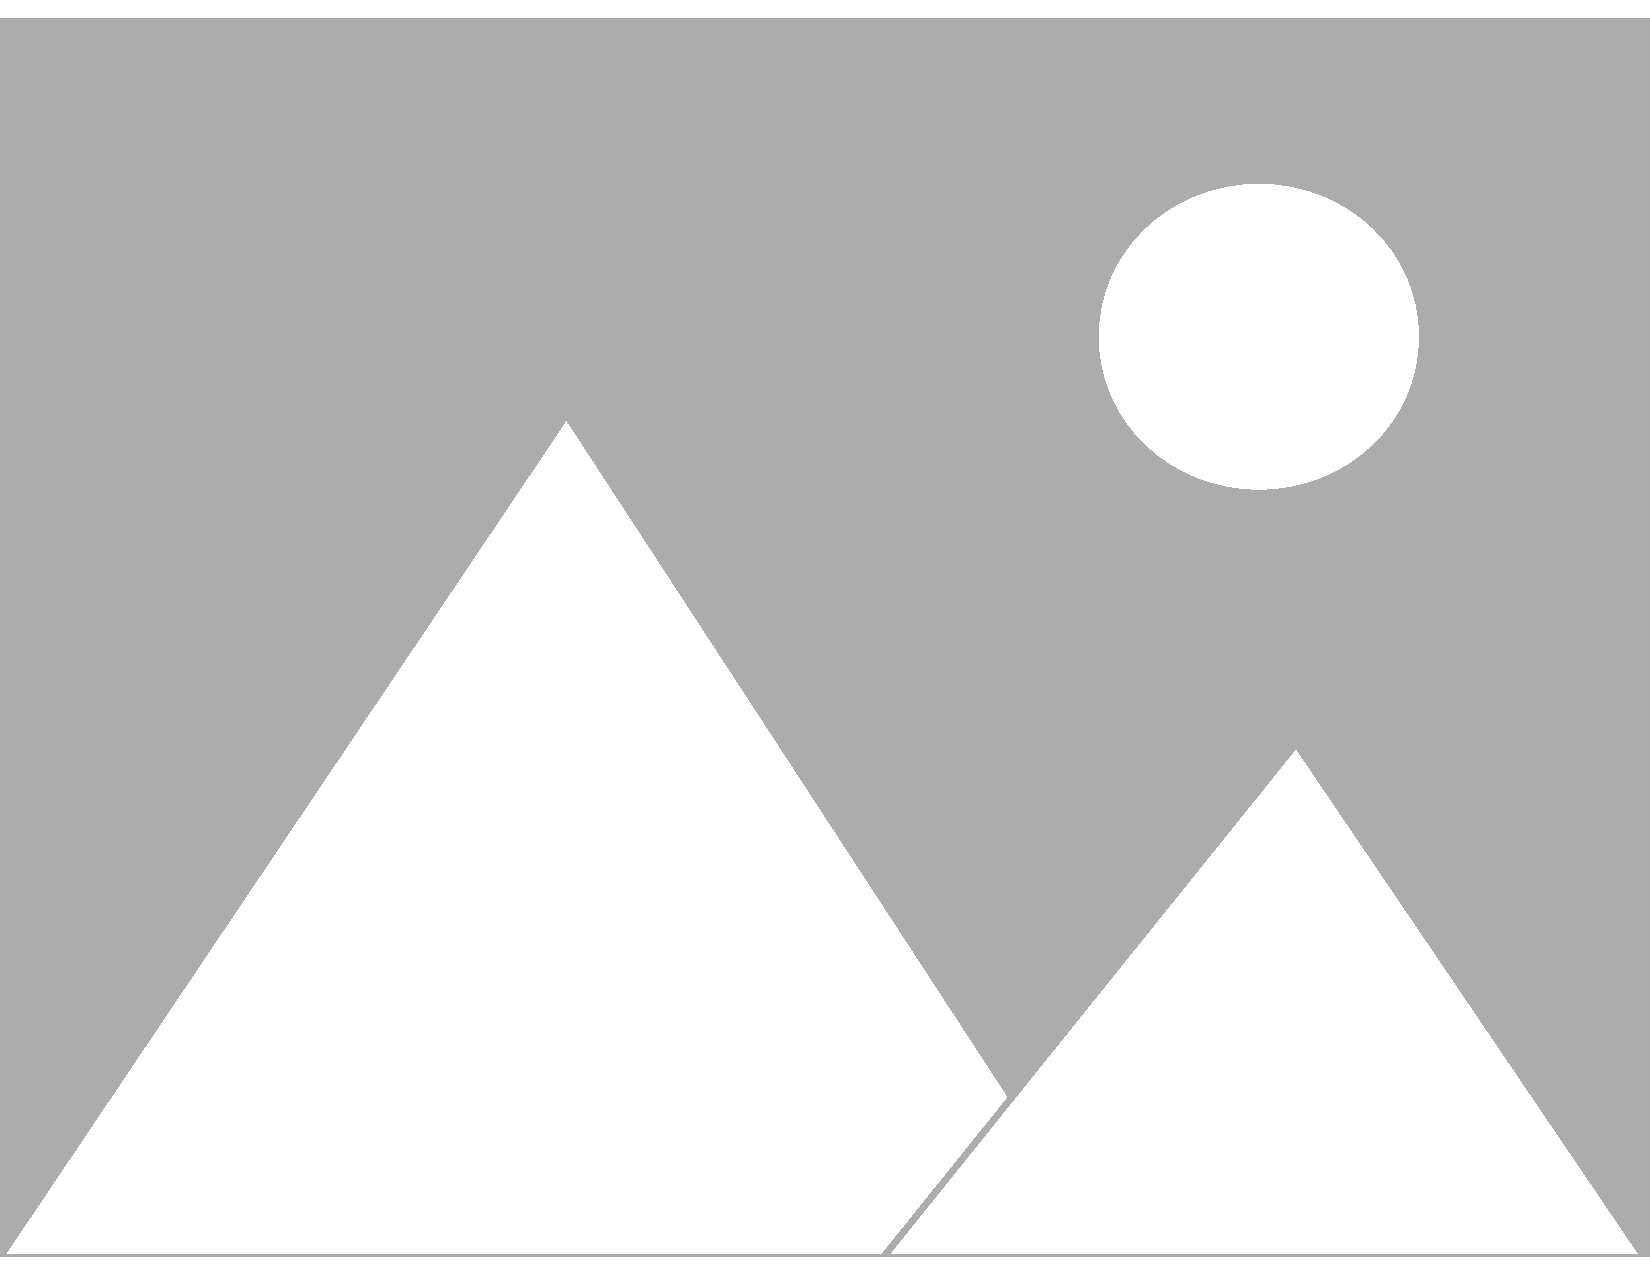
\includegraphics[width=0.5\textwidth]{figure1}
 \caption{Text describing the figure and the main conclusions drawn from it. To make your figures accessible to as many readers as possible, try to avoid using colour as the only means of conveying information. For example, in charts and graphs use different line styles and symbols. Further information is available in the online guide: \href{https://publishingsupport.iopscience.iop.org/publishing-support/authors/authoring-for-journals/writing-journal-article/\#figures}{https://publishingsupport.iopscience.iop.org/publishing-support/authors/authoring-for-journals/writing-journal-article/\#figures}}
\label{fig1}
\end{figure}


\begin{table}
\caption{Caption text describing the table. Adapt the template table below or replace with a new table. To add more tables, copy and paste the whole {\tt \textbackslash begin\{table\}...\textbackslash end\{table\}} block.}
\centering
\begin{tabular}{l c c c}
\hline
Column heading & Column heading & Column heading & Column heading \\
\hline
Data row 1 & 1.0 & 1.5 & 2.0 \\
Data row 2 & 2.0 & 2.5 & 3.0 \\
Data row 3 & 3.0 & 3.5 & 4.0 \\
\hline
\end{tabular}
\label{tab1}
\end{table}

\bibliographystyle{plain}
\bibliography{iopbib}

%
% Each of the commands below will create an unnumbered section with the appropriate heading.
% Remove any sections that are not relevant for your article.
% All sections except suppdata will be removed if the [anonymous] option is used.
% See iopjournal-guidelines.pdf for more information.
%

\ack{The author acknowledges the wildlife management organizations, state agencies, and educational institutions that provided trail camera and post-mortem dental analysis training materials used in dataset construction. Particular appreciation is extended to the wildlife professionals who developed these educational resources, enabling this interdisciplinary application of computer vision to wildlife biology. Appreciation is also extended to the open-source community for the deep learning frameworks and tools that enabled this work.}

\funding{This research received no external funding.}
% This section is a list of funder names and grant numbers

\data{Sample text inserted for demonstration.}
% For more information on IOP Publishing's research data policy see: https://publishingsupport.iopscience.iop.org/questions/research-data/

\end{document}